\documentclass[a4paper, notitlepage, fleqn]{article}

\usepackage{fullpage}
%\usepackage[cm]{fullpage}
\usepackage{glossaries}
\usepackage{algorithmicx}
\usepackage{algpseudocode}
\usepackage{amsmath}
\usepackage{mathtools}
\usepackage{hyperref}
\usepackage{amsfonts}
\usepackage{MnSymbol}
\usepackage{harpoon}
\usepackage{wrapfig}

\title{SE33010 Assignment One}
\author{Alexander D Brown (adb9)}
\newacronym{z}{Z}{Z Notation}

\begin{document}

\begin{centering}
\section*{SE33010 Assignment Two - Alexander D Brown (adb9)}
\subsection*{Moving from the Spiral Model to Formal Methods}
\end{centering}

The Spiral model of software development is a lifecycle which is intended for large, expensive and
complicated projects, explicitly including risk management as part of the development process. 
Figure~\ref{fig:spiral} depicts the overall process of the spiral model.

\begin{figure}[h]
\centering
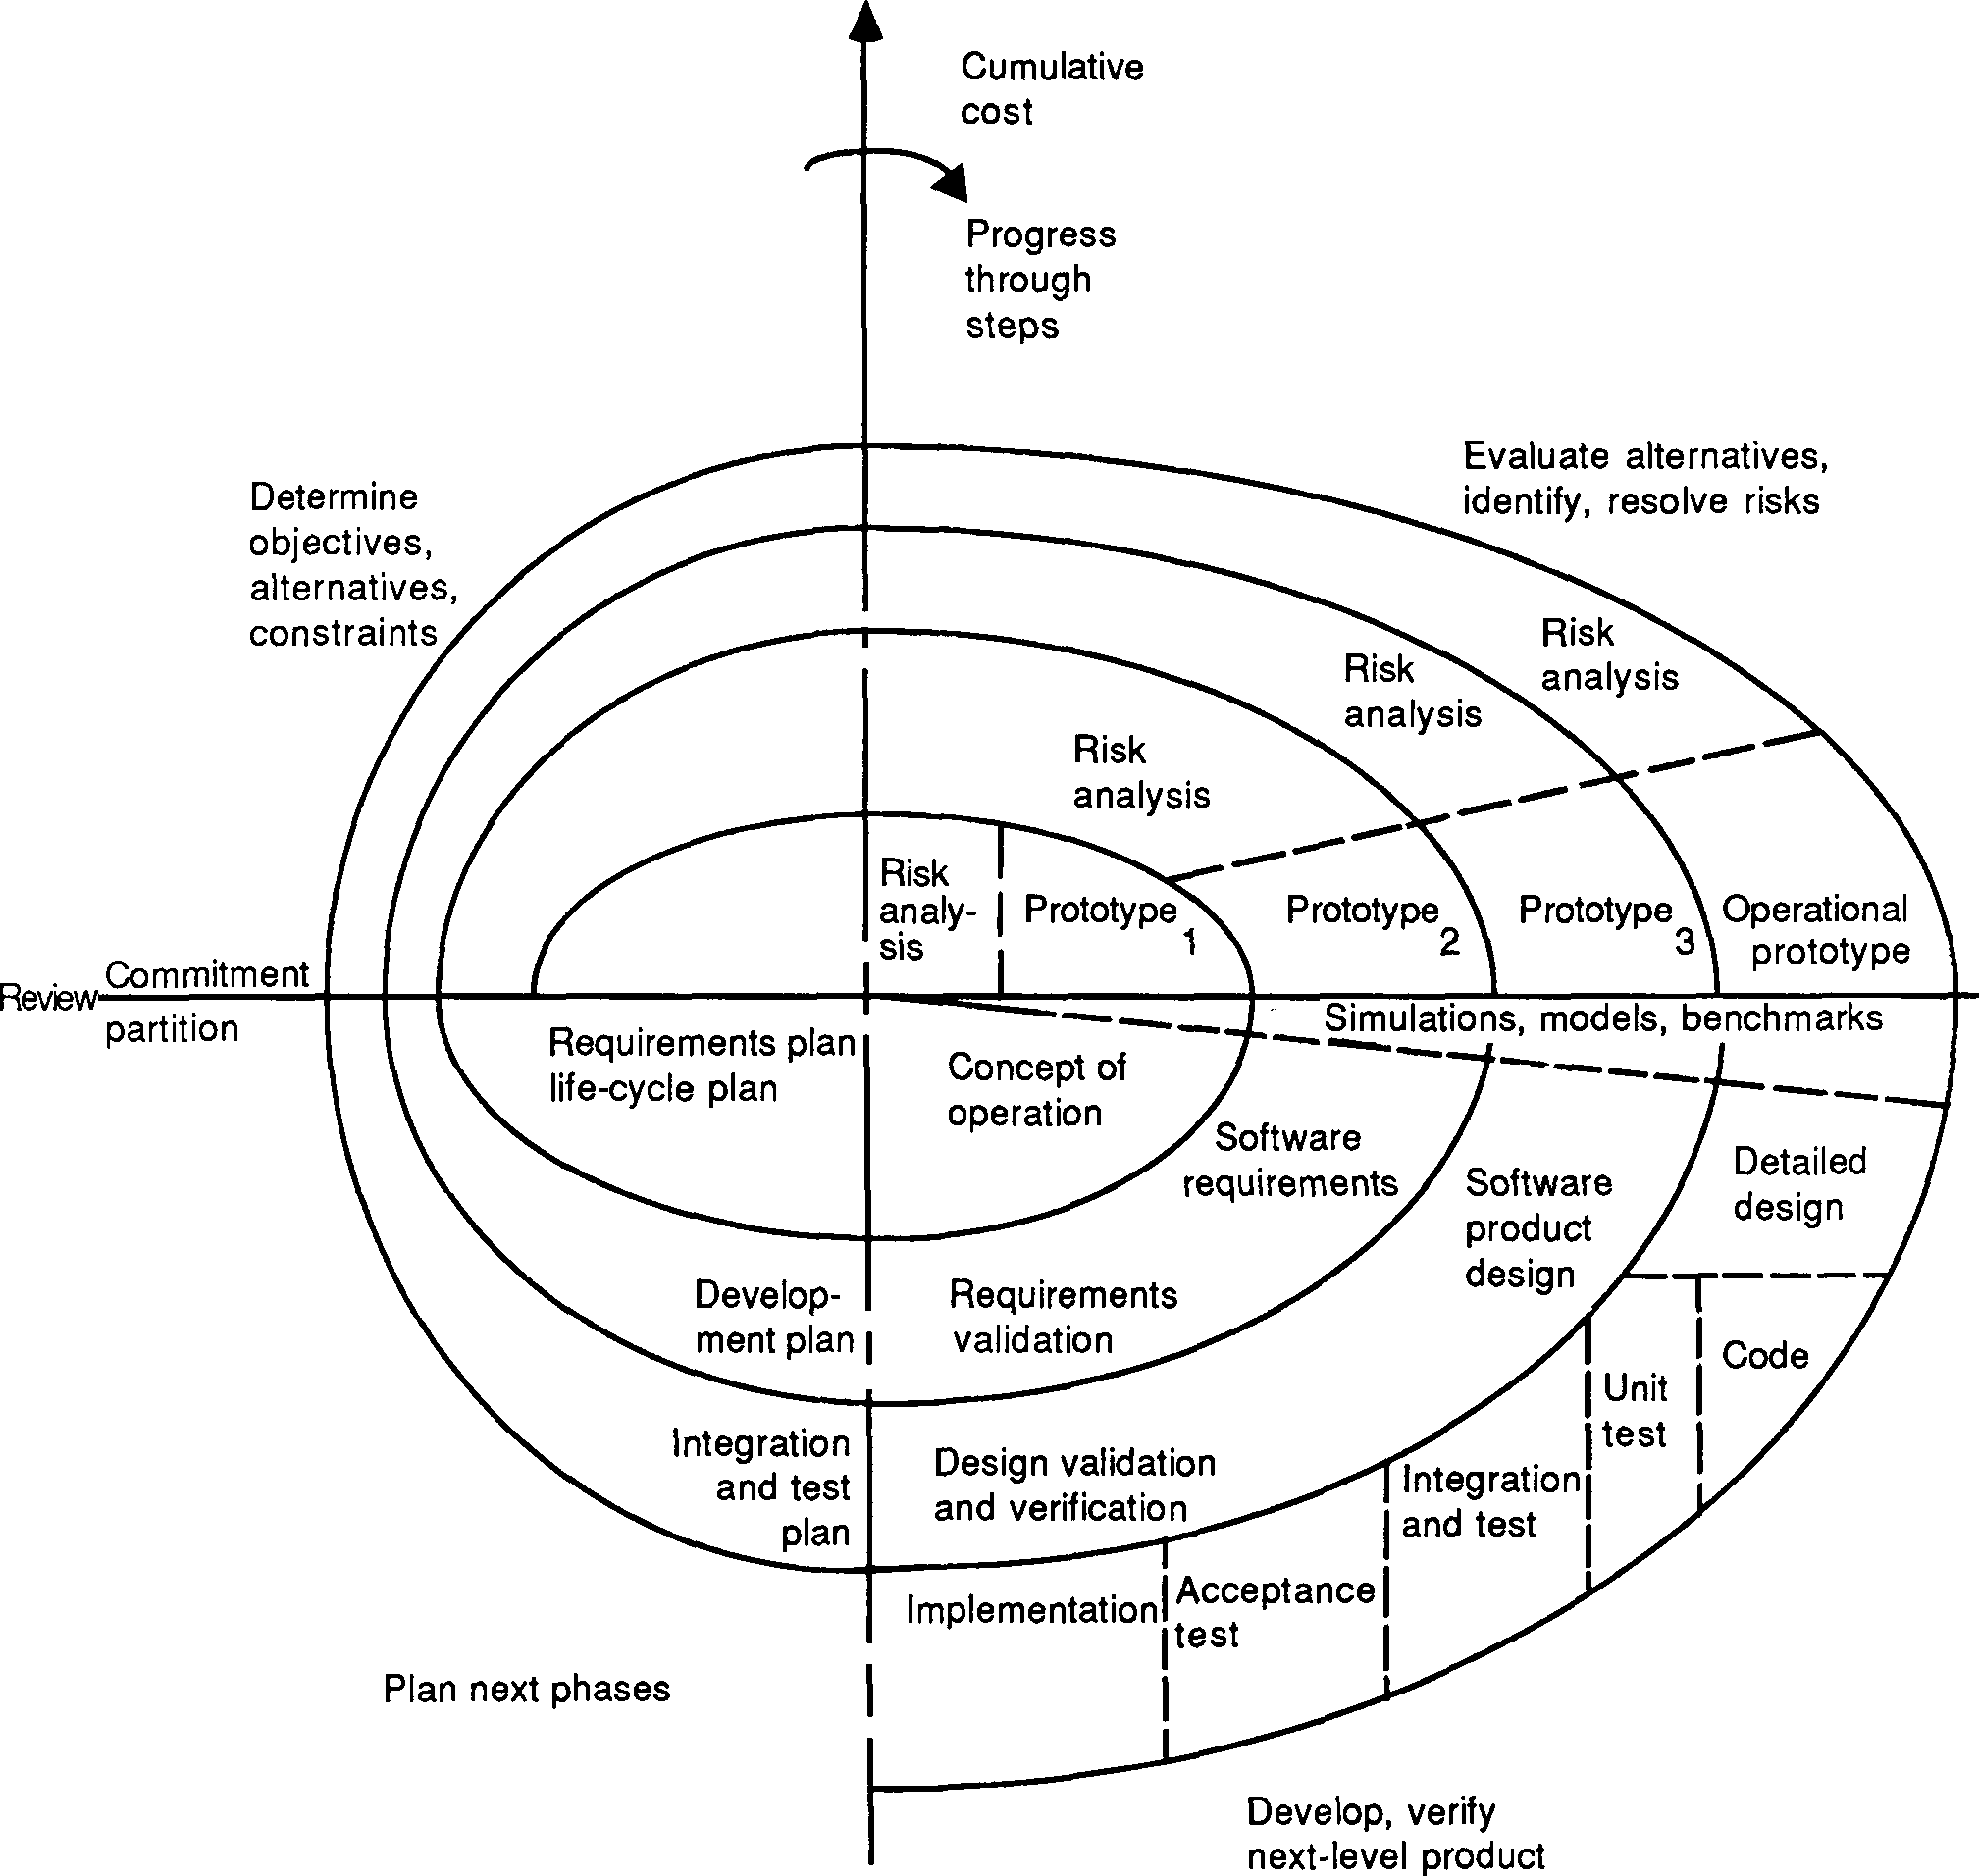
\includegraphics[width=0.4\textwidth]{img/spiral}
\caption{Spiral model of the software process\cite{59}}\label{fig:spiral}
\end{figure}

Formal Methods of software development have many different flavours but focus upon proving the
correctness of the produced software, typically through application of mathematical specification.
Formal Methods are very useful for safety- or mission- critical systems; where traditional methods
would have to rely on large amounts of testing.

Both methods start similarly; gathering requirements for the system. However the Spiral model 
focuses on both requirements and risk analysis whereas Formal Methods these requirements are used
to build an abstract specification.

This report will focus on the Vienna Development Model (VDM) as the model for a Formal Development
Method, however that are many others with different syntax or structures.

With VDM the two main focuses are on \emph{Data Reification}: the development of abstract data 
types into concrete ones and \emph{Operation Decomposition}: the development of algorithms from
the implicit specification of functions and operations.

The first change that would need to be made is to build this abstract specification based on the
requirements, defining the data types and operations which are needed to complete the system.

From this the first reification step is taken; each of these steps involve:

\begin{enumerate}
\item From the abstract data type specification $ABS$ find a new representation $REP$
\item Find a \emph{retrieve function} that relates $ABS$ to $REP$ 
%($retr: REP \rightarrow ABS$)
\item Prove that $REP$ is \emph{adequate} to represent $ABS$ 
%(prove $\forall a \in ABS \bullet \exists r \in REP \bullet a = retr(r)$)
\item Re-write functions and operations in terms of $REP$.
\item Prove that these new functions and operations preserve any data-type invariants of $REP$.
\item Prove that these new functions and operations model those of the original specification:
\begin{itemize}
\item Prove that preconditions for operation $OPA$ on $ABS$ returns the same results on 
$REP$
%:  $\forall r \in REP \bullet \mathtt{pre-}OPA(retr(r)) \Rightarrow \mathtt{pre-}OPA(r)$
\item Prove that the postconditions for operations $OPA$ on $ABS$ return the same results on $REP$
given that the preconditions were met
%: $\forall \overleftharp{r}, r \in REP \bullet \texttt{pre-}OPA(retr(\overleftharp{r})) \land \texttt{post-}OPA(\overleftharp{r},r) \Rightarrow \texttt{post-}OPA(retr(\overleftharp{r}), retr(r))$
\end{itemize}
\end{enumerate}



\bibliographystyle{plain}
\bibliography{references}

\end{document}
